% Options for packages loaded elsewhere
\PassOptionsToPackage{unicode}{hyperref}
\PassOptionsToPackage{hyphens}{url}
%
\documentclass[
]{book}
\usepackage{amsmath,amssymb}
\usepackage{iftex}
\ifPDFTeX
  \usepackage[T1]{fontenc}
  \usepackage[utf8]{inputenc}
  \usepackage{textcomp} % provide euro and other symbols
\else % if luatex or xetex
  \usepackage{unicode-math} % this also loads fontspec
  \defaultfontfeatures{Scale=MatchLowercase}
  \defaultfontfeatures[\rmfamily]{Ligatures=TeX,Scale=1}
\fi
\usepackage{lmodern}
\ifPDFTeX\else
  % xetex/luatex font selection
\fi
% Use upquote if available, for straight quotes in verbatim environments
\IfFileExists{upquote.sty}{\usepackage{upquote}}{}
\IfFileExists{microtype.sty}{% use microtype if available
  \usepackage[]{microtype}
  \UseMicrotypeSet[protrusion]{basicmath} % disable protrusion for tt fonts
}{}
\makeatletter
\@ifundefined{KOMAClassName}{% if non-KOMA class
  \IfFileExists{parskip.sty}{%
    \usepackage{parskip}
  }{% else
    \setlength{\parindent}{0pt}
    \setlength{\parskip}{6pt plus 2pt minus 1pt}}
}{% if KOMA class
  \KOMAoptions{parskip=half}}
\makeatother
\usepackage{xcolor}
\usepackage{color}
\usepackage{fancyvrb}
\newcommand{\VerbBar}{|}
\newcommand{\VERB}{\Verb[commandchars=\\\{\}]}
\DefineVerbatimEnvironment{Highlighting}{Verbatim}{commandchars=\\\{\}}
% Add ',fontsize=\small' for more characters per line
\usepackage{framed}
\definecolor{shadecolor}{RGB}{248,248,248}
\newenvironment{Shaded}{\begin{snugshade}}{\end{snugshade}}
\newcommand{\AlertTok}[1]{\textcolor[rgb]{0.94,0.16,0.16}{#1}}
\newcommand{\AnnotationTok}[1]{\textcolor[rgb]{0.56,0.35,0.01}{\textbf{\textit{#1}}}}
\newcommand{\AttributeTok}[1]{\textcolor[rgb]{0.13,0.29,0.53}{#1}}
\newcommand{\BaseNTok}[1]{\textcolor[rgb]{0.00,0.00,0.81}{#1}}
\newcommand{\BuiltInTok}[1]{#1}
\newcommand{\CharTok}[1]{\textcolor[rgb]{0.31,0.60,0.02}{#1}}
\newcommand{\CommentTok}[1]{\textcolor[rgb]{0.56,0.35,0.01}{\textit{#1}}}
\newcommand{\CommentVarTok}[1]{\textcolor[rgb]{0.56,0.35,0.01}{\textbf{\textit{#1}}}}
\newcommand{\ConstantTok}[1]{\textcolor[rgb]{0.56,0.35,0.01}{#1}}
\newcommand{\ControlFlowTok}[1]{\textcolor[rgb]{0.13,0.29,0.53}{\textbf{#1}}}
\newcommand{\DataTypeTok}[1]{\textcolor[rgb]{0.13,0.29,0.53}{#1}}
\newcommand{\DecValTok}[1]{\textcolor[rgb]{0.00,0.00,0.81}{#1}}
\newcommand{\DocumentationTok}[1]{\textcolor[rgb]{0.56,0.35,0.01}{\textbf{\textit{#1}}}}
\newcommand{\ErrorTok}[1]{\textcolor[rgb]{0.64,0.00,0.00}{\textbf{#1}}}
\newcommand{\ExtensionTok}[1]{#1}
\newcommand{\FloatTok}[1]{\textcolor[rgb]{0.00,0.00,0.81}{#1}}
\newcommand{\FunctionTok}[1]{\textcolor[rgb]{0.13,0.29,0.53}{\textbf{#1}}}
\newcommand{\ImportTok}[1]{#1}
\newcommand{\InformationTok}[1]{\textcolor[rgb]{0.56,0.35,0.01}{\textbf{\textit{#1}}}}
\newcommand{\KeywordTok}[1]{\textcolor[rgb]{0.13,0.29,0.53}{\textbf{#1}}}
\newcommand{\NormalTok}[1]{#1}
\newcommand{\OperatorTok}[1]{\textcolor[rgb]{0.81,0.36,0.00}{\textbf{#1}}}
\newcommand{\OtherTok}[1]{\textcolor[rgb]{0.56,0.35,0.01}{#1}}
\newcommand{\PreprocessorTok}[1]{\textcolor[rgb]{0.56,0.35,0.01}{\textit{#1}}}
\newcommand{\RegionMarkerTok}[1]{#1}
\newcommand{\SpecialCharTok}[1]{\textcolor[rgb]{0.81,0.36,0.00}{\textbf{#1}}}
\newcommand{\SpecialStringTok}[1]{\textcolor[rgb]{0.31,0.60,0.02}{#1}}
\newcommand{\StringTok}[1]{\textcolor[rgb]{0.31,0.60,0.02}{#1}}
\newcommand{\VariableTok}[1]{\textcolor[rgb]{0.00,0.00,0.00}{#1}}
\newcommand{\VerbatimStringTok}[1]{\textcolor[rgb]{0.31,0.60,0.02}{#1}}
\newcommand{\WarningTok}[1]{\textcolor[rgb]{0.56,0.35,0.01}{\textbf{\textit{#1}}}}
\usepackage{longtable,booktabs,array}
\usepackage{calc} % for calculating minipage widths
% Correct order of tables after \paragraph or \subparagraph
\usepackage{etoolbox}
\makeatletter
\patchcmd\longtable{\par}{\if@noskipsec\mbox{}\fi\par}{}{}
\makeatother
% Allow footnotes in longtable head/foot
\IfFileExists{footnotehyper.sty}{\usepackage{footnotehyper}}{\usepackage{footnote}}
\makesavenoteenv{longtable}
\usepackage{graphicx}
\makeatletter
\def\maxwidth{\ifdim\Gin@nat@width>\linewidth\linewidth\else\Gin@nat@width\fi}
\def\maxheight{\ifdim\Gin@nat@height>\textheight\textheight\else\Gin@nat@height\fi}
\makeatother
% Scale images if necessary, so that they will not overflow the page
% margins by default, and it is still possible to overwrite the defaults
% using explicit options in \includegraphics[width, height, ...]{}
\setkeys{Gin}{width=\maxwidth,height=\maxheight,keepaspectratio}
% Set default figure placement to htbp
\makeatletter
\def\fps@figure{htbp}
\makeatother
\setlength{\emergencystretch}{3em} % prevent overfull lines
\providecommand{\tightlist}{%
  \setlength{\itemsep}{0pt}\setlength{\parskip}{0pt}}
\setcounter{secnumdepth}{5}
\usepackage{booktabs}
\usepackage{amsthm}
\makeatletter
\def\thm@space@setup{%
  \thm@preskip=8pt plus 2pt minus 4pt
  \thm@postskip=\thm@preskip
}
\makeatother
\ifLuaTeX
  \usepackage{selnolig}  % disable illegal ligatures
\fi
\usepackage[]{natbib}
\bibliographystyle{apalike}
\IfFileExists{bookmark.sty}{\usepackage{bookmark}}{\usepackage{hyperref}}
\IfFileExists{xurl.sty}{\usepackage{xurl}}{} % add URL line breaks if available
\urlstyle{same}
\hypersetup{
  pdftitle={Notas de matemáticas},
  pdfauthor={Hector Henry Jurado Soto},
  hidelinks,
  pdfcreator={LaTeX via pandoc}}

\title{Notas de matemáticas}
\author{Hector Henry Jurado Soto}
\date{2024-03-16}

\usepackage{amsthm}
\newtheorem{theorem}{Theorem}[chapter]
\newtheorem{lemma}{Lemma}[chapter]
\newtheorem{corollary}{Corollary}[chapter]
\newtheorem{proposition}{Proposition}[chapter]
\newtheorem{conjecture}{Conjecture}[chapter]
\theoremstyle{definition}
\newtheorem{definition}{Definition}[chapter]
\theoremstyle{definition}
\newtheorem{example}{Example}[chapter]
\theoremstyle{definition}
\newtheorem{exercise}{Exercise}[chapter]
\theoremstyle{definition}
\newtheorem{hypothesis}{Hypothesis}[chapter]
\theoremstyle{remark}
\newtheorem*{remark}{Remark}
\newtheorem*{solution}{Solution}
\begin{document}
\maketitle

{
\setcounter{tocdepth}{1}
\tableofcontents
}
\hypertarget{prerequisites}{%
\chapter{Prerequisites}\label{prerequisites}}

This is a \emph{sample} book written in \textbf{Markdown}. You can use anything that Pandoc's Markdown supports, e.g., a math equation \(a^2 + b^2 = c^2\).

The \textbf{bookdown} package can be installed from CRAN or Github:

\begin{Shaded}
\begin{Highlighting}[]
\FunctionTok{install.packages}\NormalTok{(}\StringTok{"bookdown"}\NormalTok{)}
\CommentTok{\# or the development version}
\CommentTok{\# devtools::install\_github("rstudio/bookdown")}
\end{Highlighting}
\end{Shaded}

Remember each Rmd file contains one and only one chapter, and a chapter is defined by the first-level heading \texttt{\#}.

To compile this example to PDF, you need XeLaTeX. You are recommended to install TinyTeX (which includes XeLaTeX): \url{https://yihui.name/tinytex/}.

\hypertarget{intro}{%
\chapter{Introduction}\label{intro}}

You can label chapter and section titles using \texttt{\{\#label\}} after them, e.g., we can reference Chapter \ref{intro}. If you do not manually label them, there will be automatic labels anyway, e.g., Chapter \ref{methods}.

Figures and tables with captions will be placed in \texttt{figure} and \texttt{table} environments, respectively.

\begin{Shaded}
\begin{Highlighting}[]
\FunctionTok{par}\NormalTok{(}\AttributeTok{mar =} \FunctionTok{c}\NormalTok{(}\DecValTok{4}\NormalTok{, }\DecValTok{4}\NormalTok{, .}\DecValTok{1}\NormalTok{, .}\DecValTok{1}\NormalTok{))}
\FunctionTok{plot}\NormalTok{(pressure, }\AttributeTok{type =} \StringTok{\textquotesingle{}b\textquotesingle{}}\NormalTok{, }\AttributeTok{pch =} \DecValTok{19}\NormalTok{)}
\end{Highlighting}
\end{Shaded}

\begin{figure}

{\centering 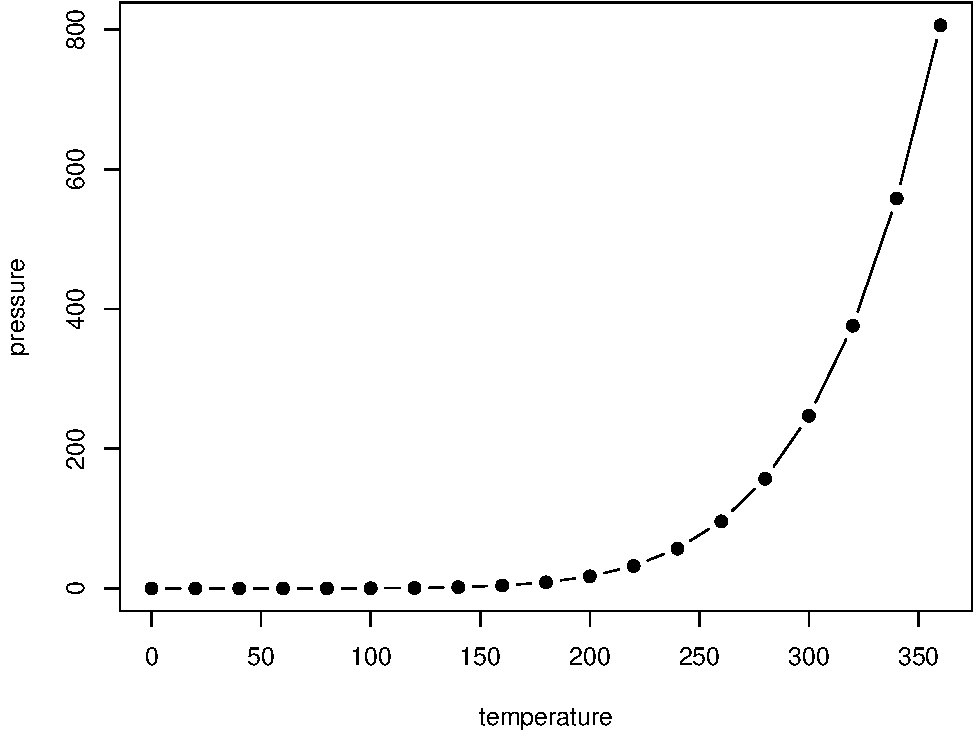
\includegraphics[width=0.8\linewidth]{bookdown-demo_files/figure-latex/nice-fig-1} 

}

\caption{Here is a nice figure!}\label{fig:nice-fig}
\end{figure}

Reference a figure by its code chunk label with the \texttt{fig:} prefix, e.g., see Figure \ref{fig:nice-fig}. Similarly, you can reference tables generated from \texttt{knitr::kable()}, e.g., see Table \ref{tab:nice-tab}.

\begin{Shaded}
\begin{Highlighting}[]
\NormalTok{knitr}\SpecialCharTok{::}\FunctionTok{kable}\NormalTok{(}
  \FunctionTok{head}\NormalTok{(iris, }\DecValTok{20}\NormalTok{), }\AttributeTok{caption =} \StringTok{\textquotesingle{}Here is a nice table!\textquotesingle{}}\NormalTok{,}
  \AttributeTok{booktabs =} \ConstantTok{TRUE}
\NormalTok{)}
\end{Highlighting}
\end{Shaded}

\begin{table}

\caption{\label{tab:nice-tab}Here is a nice table!}
\centering
\begin{tabular}[t]{rrrrl}
\toprule
Sepal.Length & Sepal.Width & Petal.Length & Petal.Width & Species\\
\midrule
5.1 & 3.5 & 1.4 & 0.2 & setosa\\
4.9 & 3.0 & 1.4 & 0.2 & setosa\\
4.7 & 3.2 & 1.3 & 0.2 & setosa\\
4.6 & 3.1 & 1.5 & 0.2 & setosa\\
5.0 & 3.6 & 1.4 & 0.2 & setosa\\
\addlinespace
5.4 & 3.9 & 1.7 & 0.4 & setosa\\
4.6 & 3.4 & 1.4 & 0.3 & setosa\\
5.0 & 3.4 & 1.5 & 0.2 & setosa\\
4.4 & 2.9 & 1.4 & 0.2 & setosa\\
4.9 & 3.1 & 1.5 & 0.1 & setosa\\
\addlinespace
5.4 & 3.7 & 1.5 & 0.2 & setosa\\
4.8 & 3.4 & 1.6 & 0.2 & setosa\\
4.8 & 3.0 & 1.4 & 0.1 & setosa\\
4.3 & 3.0 & 1.1 & 0.1 & setosa\\
5.8 & 4.0 & 1.2 & 0.2 & setosa\\
\addlinespace
5.7 & 4.4 & 1.5 & 0.4 & setosa\\
5.4 & 3.9 & 1.3 & 0.4 & setosa\\
5.1 & 3.5 & 1.4 & 0.3 & setosa\\
5.7 & 3.8 & 1.7 & 0.3 & setosa\\
5.1 & 3.8 & 1.5 & 0.3 & setosa\\
\bottomrule
\end{tabular}
\end{table}

You can write citations, too. For example, we are using the \textbf{bookdown} package \citep{R-bookdown} in this sample book, which was built on top of R Markdown and \textbf{knitr} \citep{xie2015}.

Mi referencia \citep{blitzstein2019}.

\hypertarget{literature}{%
\chapter{Literature}\label{literature}}

Here is a review of existing methods.

\hypertarget{methods}{%
\chapter{Methods}\label{methods}}

We describe our methods in this chapter.

Math can be added in body using usual syntax like this

\hypertarget{math-example}{%
\section{math example}\label{math-example}}

\(p\) is unknown but expected to be around 1/3. Standard error will be approximated

\[
SE = \sqrt(\frac{p(1-p)}{n}) \approx \sqrt{\frac{1/3 (1 - 1/3)} {300}} = 0.027
\]

You can also use math in footnotes like this\footnote{where we mention \(p = \frac{a}{b}\)}.

We will approximate standard error to 0.027\footnote{\(p\) is unknown but expected to be around 1/3. Standard error will be approximated

  \[
  SE = \sqrt(\frac{p(1-p)}{n}) \approx \sqrt{\frac{1/3 (1 - 1/3)} {300}} = 0.027
  \]}

\hypertarget{applications}{%
\chapter{Applications}\label{applications}}

Some \emph{significant} applications are demonstrated in this chapter.

\hypertarget{example-one}{%
\section{Example one}\label{example-one}}

\hypertarget{example-two}{%
\section{Example two}\label{example-two}}

\hypertarget{final-words}{%
\chapter{Final Words}\label{final-words}}

We have finished a nice book.

\hypertarget{probabilidad}{%
\chapter{Probabilidad}\label{probabilidad}}

\hypertarget{espacios-muestrales}{%
\section{Espacios muestrales}\label{espacios-muestrales}}

\begin{definition}[Espacio muestral y evento]
\protect\hypertarget{def:muestral}{}\label{def:muestral}El \emph{espacio muestral} \(S\) de un experimento es el conjunto de todos los posibles resultados de un experimento. Un \emph{evento} \(A\) es un subconjunto del espacio muestral \(S\) y se dice que \(A\) \emph{ocurrió} si el resultado actual pertenece a \(A\)
\end{definition}

\citep{blitzstein2019}

\begin{figure}

{\centering 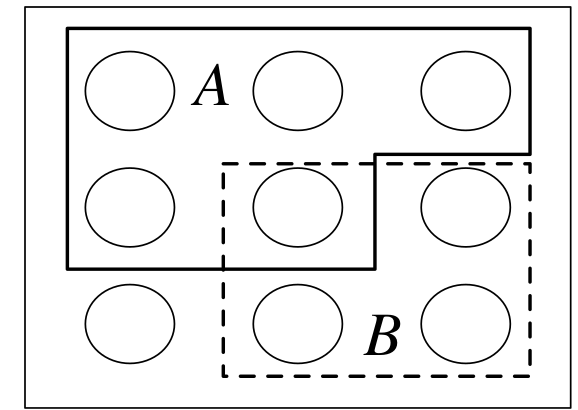
\includegraphics[width=0.3\linewidth]{./images/pebbles} 

}

\caption{Un espacio muestral es como  un mundo de canicas con dos eventos $A$ y $B$}\label{fig:unnamed-chunk-3}
\end{figure}

El espacio muestral de un experimento puede ser finito o infinito contable o infinito incontable, cuando el espacio muestral es finito puede visualizarse como un mundo de canicas, como muestra la figura. Cada canica representa un resultado, y un evento es un conjunto de canicas. Realizar un experimento es equivalente a escoger una canica en forma aleatoria.

Por ejemplo, sea \(S\) el espacio muestral de un experimento y sean \(A\) y \(B\) eventos. Entonces, la unión \(A \cup B\) es el evento que ocurre si y solo si al menos uno de \(A\) y \(B\) ocurre, la intersección \(A \cap B\) es el evento que ocurre si y solo si ambos \(A\) y \(B\) ocurren, y el complemento \(A^c\) es el evento que ocurre si y solo si \(A\) no ocurre. También tenemos las leyes de De Morgan:

\[(A \cup B)^c = A^c \cap B^c \textrm{ and } (A \cap B)^c = A^c \cup B^c\]

puesto que decir que no es el caso que al menos uno de \(A\) y \(B\) ocurra es lo mismo que decir que \(A^c\) no ocurre y \(B^c\) no ocurre, y decir que no es el caso que ambos ocurran es lo mismo que decir que al menos uno no ocurre. Resultados análogos se mantienen para uniones e intersecciones de más de dos eventos.

En el ejemplo mostrado en la Figura, \(A\) es un conjunto de \(n\) canicas, \(B\) es un conjunto de \(m\) canicas, \(A \cup B\) consiste en los \(n + m\) canicas en \(A\) o \(B\) (incluyendo el canicas que está en ambos), \(A \cap B\) consiste en las canicas que está en ambos \(A\) y \(B\), y \(A^c\) consiste en las \(n\) canicas que no están en \(A\).

En el ejemplo de la figura, \(A\) es un conjunto de 5 canicas,\(B\) es un conjunto de 4 canicas, \(A \cup B\) es un conjunto de 8 canicas, incluyendo la que esta en los dos conjuntos, \(A \cap B\) es un conjunto de 1 canica y \(A^c\) consiste en cuatro canicas que no están en \(A\)

\begin{example}[Espacio muestral y evento]
\protect\hypertarget{exm:coins}{}\label{exm:coins}Una moneda es lanzada 10 veces , se escribirá heads como \(H\) y tails como \(T\), un posible resultado es \(HHHTHHTTHT\), el espacio muestral es el conjunto de todas las posibles cadenas de longitud 10 de \(H's\) y \(T's\).

Se puede codificar \(H\) como \(1\) y \(T\) como \(0\), asi que un resultado es una secuencia \((s_1,s_2,s_3, ..., s_{10}))\) con \(s_j \in \{0, 1\}\), y el espacio muestral es el conjunto de todas esas secuencias.

Veamos ahora algunos eventos:

\begin{enumerate}
\def\labelenumi{\arabic{enumi}.}
\tightlist
\item
  Sea \(A_1\) el evento en que la primer lanzamiento es Head
\end{enumerate}

\[ A_1 = {(1,s_2, ...,s_{10}) }: s_j \in\ \{0,1\} , 2 \leq j  \leq  10\]

Este es un subconjunto del espacio muestral, o sea un evento, decir que \(A_1\) ocurre es lo mismo que decir que el primer lanzamiento es Head. Similarmente se dice que \(A_j\) es el evento en que el \(j_{esimo}\) lanzamiento es Head, donde j =2,3,\ldots,10.

\begin{enumerate}
\def\labelenumi{\arabic{enumi}.}
\setcounter{enumi}{1}
\item
  Sea \(B\) el evento en el que al menos un lanzamiento fue head \[ B =   \bigcup_{j=1}^{10} A_j  \]
\item
  Sea \(C\) el evento en el que todos los lanzamientos fueron heads \[ C =   \bigcap_{j=1}^{10} A_j  \]
\item
  Sea \(D\) el evento en que hubo al menos dos Heads consecutivos
\end{enumerate}

\[ C =   \bigcup_{j=1}^{9} ( A_j \cap A_{j+1} )   \]
\end{example}

\hypertarget{definicion-ingenua-de-probabilidad-naive-definition-of-probability}{%
\section{Definicion ingenua de probabilidad (Naive definition of probability)}\label{definicion-ingenua-de-probabilidad-naive-definition-of-probability}}

Históricamente, la definición de probabilidad de un evento fue contar el número de maneras en que evento puede suceder y dividir por el número total de resultados posibles del experimento.

\begin{definition}[Definición ingenua de probabilidad]
\protect\hypertarget{def:definicioningenuaprobabilidad}{}\label{def:definicioningenuaprobabilidad}Sea \(A\) un evento para un experimento con un espacio muestral finito \(S\) . la probabilidad ingenua de \(A\) es

\[P_{naive} (A) = \frac{|A|}{|S|} = \frac { numero\, de\, resultados\, favorables\, de\, A}{total\, numero\, de\, resultados\, en\, S} \]

en donde \textbar A\textbar{} es el tamaño (cardinalidad ) del conjunto A
\end{definition}

La definición ingenua es muy restrictiva en que esto requiere que \(S\) sea finito, con igual masa para cada uno de las canicas por ejemplo. A a menudo es mal aplicado por personas que asumen resultados igualmente probables sin justificación y presentan argumentos en el sentido de '' o sucederá o no sucederá y no sabemos cual, así que es 50-50''. Por ejemplo, si no sabemos si hay vida en saturno ¿deberíamos concluir que es 50-50? ¿Que pasa con la vida inteligente en saturno, que parece que debería ser estrictamente menos probable que exista alguna forma de vida en saturno ? Sin embargo hay varios tipos importantes de problemas en los que la definición ingenua es aplicable, como cuando hay simetría en el problema, que hace que los resultados sean igualmente probables.\citep{blitzstein2019}

\hypertarget{probabilidad-y-conteo}{%
\section{Probabilidad y conteo}\label{probabilidad-y-conteo}}

Calcular la probabilidad ingenua de un evento \(A\) implica contar el numero de canicas en \(A\) y el numero de canicas en el espacio muestral \(S\). A menudo estos conjuntos con extremadamente grandes, por lo que podría ser tedioso o inviable contar las posibilidades uno a uno. Para abordar este desafío existen algunas técnicas de conteo.

\begin{theorem}[Regla de la multiplicación]
\protect\hypertarget{thm:reglamultiplicacion}{}\label{thm:reglamultiplicacion}Consideremos un experimento compuesto consistiendo en dos sub-experimentos, experimento \(A\) y experimento \(B\). supongamos que el experimiento \(A\) tiene \(a\) posibles resultados y para cada uno de esos resultados el experimento \(B\) tiene \(b\) posibles resultados, entonces el experimento compuesto tiene \(ab\) posibles resultados
\end{theorem}

Imaginemos un diagrama como muestra la figura, consta de

\begin{example}[conos de helado]
\protect\hypertarget{exm:ejemplomultiplicacion}{}\label{exm:ejemplomultiplicacion}Supongamos que estamos comprando un helado en cono, se puede escoger entre un cake(pastel) o un waffle(oblea) y cada uno de ellos puede tener chocolate , vainilla o fresa como su sabor
\end{example}

\begin{figure}

{\centering 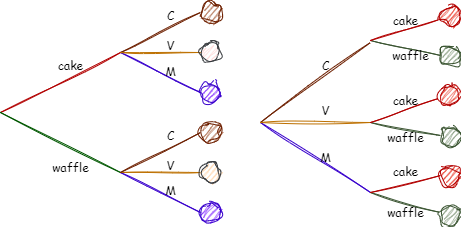
\includegraphics[width=0.8\linewidth]{./images/reglademultiplicacion1.drawio} 

}

\caption{Diagrama de árbol para un cono de helado}\label{fig:unnamed-chunk-4}
\end{figure}

Por la regla de la multiplicación existen \(2.3=3.2=6\) posibilidades. Pero debemos tener en cuenta algunas cosas como:

\begin{itemize}
\item
  No importa si se elige primero el tipo de cono ( ``quiero un cono de waffles con helado de chocolate'' ) o el sabor (``Quiero un cono de chocolate en un cono de waffles''), de cualquier forma hay posibilidades.
\item
  No importa si los mismos sabores están disponibles en un cono de pastel que en un cono de oblea, Lo que importa es que hay exactamente tres opciones de sabor para cada opción de cono, si por algún motivo estuviese prohibido tener un sabor de chocolate en un cono de oblea por ejemplo ( y sin sustituto, ) , hay posibilidades pero la regla de multiplicación no aplicaría.
\end{itemize}

Podemos usar la regla de multiplicación para llegar a fórmulas de muestreo con y sin reemplazo. Muchos experimentos en probabilidad y estadística pueden interpretarse en un de estos dos contextos, por lo que es atractivo que ambas fórmulas seigan directamente el mismo principio básico de conteo.

\begin{theorem}[Muestreo con reemplazo]
\protect\hypertarget{thm:muestreoconreemplazo}{}\label{thm:muestreoconreemplazo}Consideremos \(n\) objetos y tomamos \(k\) de ellos, una a la vez con reemplazo( es decir elegir un determinado objeto no impide que se elija nuevamente). entonces hay \(n^k\) posibles resultados
\end{theorem}

Por ejemplo, imaginemos que un frasco con \(n\) canicas, etiquetadas del 1 a \(n\), tomamos muestras de las bolas, una a la vez con reemplazo, lo que significa que cada vez que se elige una bola, se devuelve al frasco. Cada bola muestreada es un sub-experimento con \(n\) posibles resultados, y hay \(k\) sub-experimentos, entonces mediante la regla de multiplicación , hay \(n^k\) formas de obtener una muestra de tamaño \(k\)

\begin{figure}

{\centering 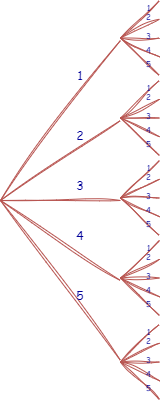
\includegraphics[width=2.25in]{./images/muestreoconreemplazo.drawio} 

}

\caption{Muestreo con reemplazo cuando n=5 y k = 2}\label{fig:unnamed-chunk-5}
\end{figure}

\begin{theorem}[Muestreo sin reemplazo]
\protect\hypertarget{thm:muestreosinreemplazo}{}\label{thm:muestreosinreemplazo}Consideremos \(n\) objetos y tomamos \(k\) de ellos, una a la vez sin reemplazo( es decir elegir un determinado objeto y se impide que se elija nuevamente). entonces hay \(n(n-1) ... (n-k+1)\) posibles resultados , para \(k <= n\) y (0 posibilidades para \(k>n\))
\end{theorem}

\begin{figure}

{\centering 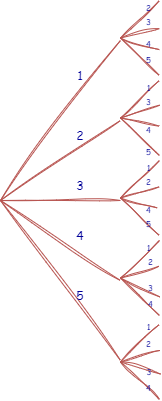
\includegraphics[width=2.25in]{./images/muestreosinreemplazo.drawio} 

}

\caption{Muestreo sin reemplazo cuando n=5 y k = 2}\label{fig:unnamed-chunk-6}
\end{figure}

El resultado es consecuencia directa de la regla de multiplicación: cada canica muestreada es otra vez un sub-experimento, y el número de posibles resultados decrece en uno (1) cada vez. Notemos que para muestrear \(k\) de \(n\) objetos sin reemplazo, necesitamos \(k <= n\), mientras que en el muestreo con reemplazo los objetos son inagotables.

\begin{example}[Permutaciones y factoriales]
\protect\hypertarget{exm:permutaciones}{}\label{exm:permutaciones}Una \emph{permutación} de \(1,2,...,n\) es una disposicion de ellos en algun orden, ej. \(3,5,1,2,4\) es una permutación de \(1,2,3,4,5\) por el teorema \ref{thm:muestreosinreemplazo} con \(k=n\) tendríamos que hay \(n!\) permutaciones de \(1,2,...,n\). Por ejemplo hay \(n!\) maneras en las cuales \(n\) personas pueden alinearse en una fila para comprar un helado
\end{example}

Los teoremas \ref{thm:muestreoconreemplazo} y \ref{thm:muestreosinreemplazo} se refieren a \emph{conteo}, pero cuando la definición de probabilidad ingenua aplica, podemos usarlos para calcular \emph{probabilidades}

\begin{example}[Problema del nacimiento]
\protect\hypertarget{exm:problemanacimiento}{}\label{exm:problemanacimiento}Existen \(k\) personas en un cuarto, asumimos que los cumpleaños de cada persona son igualmente probables para cualquiera de los 365 días del año (se excluye febrero 29), y que los cumpleaños son independientes ( no hay gemelos en el cuarto), cual es la probabilidad que dos o mas personas en el grupo tengan la misma fecha de cumpleaños.
\end{example}

\textbf{Solución}
La definición de probabilidad ingenua dice que solo necesitamos contar el numero de formas para asignar cumpleaños a \$k4 personas de tal forma que hay dos o mas personas comparten la misma fecha de cumpleaños. Este problema de conteo es un poco complejo, puesto que por ejemplo Emma y Steve comparten la fecha de cumpleaños, o Steve y Naomi o los tres juntos, o tres de ellos pueden compartir la fecha de cumpleaños, mientras otros dos en el grupo comparten fecha de nacimiento diferentes, o un monton de otras posibilidades.

En vez de eso, contemos el complemento: el numero de maneras para asignar cumpleaños a \(k\) personas de tal forma que no haya dos personas que compartan un cumpleaños. Esto equivale a un muestreo de los 365 dias del año \emph{sin} reemplazo, es decir para la primera persona, hay 365 opciones para elegir el día del año de su cumpleaños, para la segunda persona, quedan 364 opciones, ya que no puede compartir el mismo día de cumpleaños con la primera persona. De manera similar, para la tercera persona quedan 363 opciones, puesto que no puede compartir el mismo día de cumpleaños con las dos primeras personas, de igual forma para la \(k-esima\) persona hay \(365-k+1\) opciones, por lo tanto el numero total de formas de asignar cumpleaños es por el teorema \ref{thm:muestreosinreemplazo} de \(365.364.363...(365-k+1)\) para \(k<=365\)

Sea \(A\) el evento de obtener formas en que todas \(k\) personas cumplen años en días diferentes, por tanto \(|A|=365.364.363...(365-k+1)\)

El total de formas posibles de asignar cumpleaños en el cuarto es \(|S|=365^k\), a las \(k\) personas, ya que cada persona puede tener su cumpleaños en cualquiera de los 365 días del año, de acuerdo al teorema \ref{thm:muestreoconreemplazo}

por tanto :

\[P(A)=\frac{|A|}{|B|} =\frac{365.364.363...(365-k+1)}{365^k}  \]

\[P(A)=\frac{|A|}{|B|} =\frac{365.364.363...(365-k+1)}{365^k}  \]
Por tanto la probabilidad de que al menos una fecha de cumpleaños coincida es;
\[1 - P(A) = 1- \frac{365.364.363...(365-k+1)}{365^k}  \]
La figura realizada con python dibuja la probabilidad de que al menos una fecha de cumpleaños concuerda como una funcion de \(k\). con \(k=23\) la probabilidad de coincidencia excede \(0.5\), para \(k=57\) la probabilidad es cercana al \%99\%

\begin{figure}

{\centering 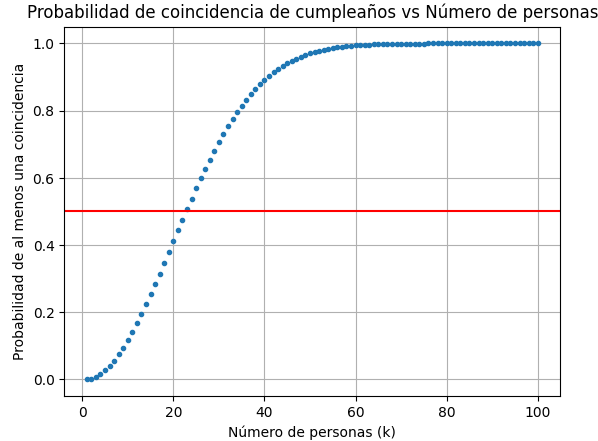
\includegraphics[width=0.6\linewidth]{./images/paradojacumpleanos} 

}

\caption{Probabilidad de  que en un cuarto de $k$ personas al menos dos nacen en el mismo día}\label{fig:unnamed-chunk-7}
\end{figure}

\hypertarget{codigos-fuente}{%
\chapter*{Codigos fuente}\label{codigos-fuente}}
\addcontentsline{toc}{chapter}{Codigos fuente}

\begin{Shaded}
\begin{Highlighting}[]
\ImportTok{import}\NormalTok{ matplotlib.pyplot }\ImportTok{as}\NormalTok{ plt}
\KeywordTok{def}\NormalTok{ calcular\_probabilidad(k):}
\NormalTok{    numerador }\OperatorTok{=} \DecValTok{1}
    \ControlFlowTok{for}\NormalTok{ i }\KeywordTok{in} \BuiltInTok{range}\NormalTok{(}\DecValTok{365} \OperatorTok{{-}}\NormalTok{ k }\OperatorTok{+} \DecValTok{1}\NormalTok{, }\DecValTok{366}\NormalTok{):}
\NormalTok{        numerador }\OperatorTok{*=}\NormalTok{ i}
\NormalTok{    denominador }\OperatorTok{=} \DecValTok{365} \OperatorTok{**}\NormalTok{ k}
    \ControlFlowTok{return} \DecValTok{1} \OperatorTok{{-}}\NormalTok{ numerador }\OperatorTok{/}\NormalTok{ denominador}

\NormalTok{k\_values }\OperatorTok{=} \BuiltInTok{list}\NormalTok{(}\BuiltInTok{range}\NormalTok{(}\DecValTok{1}\NormalTok{, }\DecValTok{100}\NormalTok{))  }\CommentTok{\# Valores de k de 1 a 100}


\NormalTok{probabilidades }\OperatorTok{=}\NormalTok{ [calcular\_probabilidad(k) }\ControlFlowTok{for}\NormalTok{ k }\KeywordTok{in}\NormalTok{ k\_values]}

\NormalTok{plt.plot(k\_values, probabilidades, marker}\OperatorTok{=}\StringTok{\textquotesingle{}.\textquotesingle{}}\NormalTok{, linestyle}\OperatorTok{=}\StringTok{\textquotesingle{}\textquotesingle{}}\NormalTok{)}
\NormalTok{plt.xlabel(}\StringTok{\textquotesingle{}Número de personas (k)\textquotesingle{}}\NormalTok{)}
\NormalTok{plt.ylabel(}\StringTok{\textquotesingle{}Probabilidad de al menos una coincidencia\textquotesingle{}}\NormalTok{)}
\NormalTok{plt.title(}\StringTok{\textquotesingle{}Probabilidad de coincidencia de cumpleaños vs Número de personas\textquotesingle{}}\NormalTok{)}
\NormalTok{plt.grid(}\VariableTok{True}\NormalTok{)}
\CommentTok{\# Línea en el 50\%}
\NormalTok{plt.axhline(y}\OperatorTok{=}\FloatTok{0.5}\NormalTok{, color}\OperatorTok{=}\StringTok{\textquotesingle{}r\textquotesingle{}}\NormalTok{, linestyle}\OperatorTok{=}\StringTok{\textquotesingle{}{-}\textquotesingle{}}\NormalTok{)}
\NormalTok{plt.show()}
\end{Highlighting}
\end{Shaded}

\begin{figure}
\centering
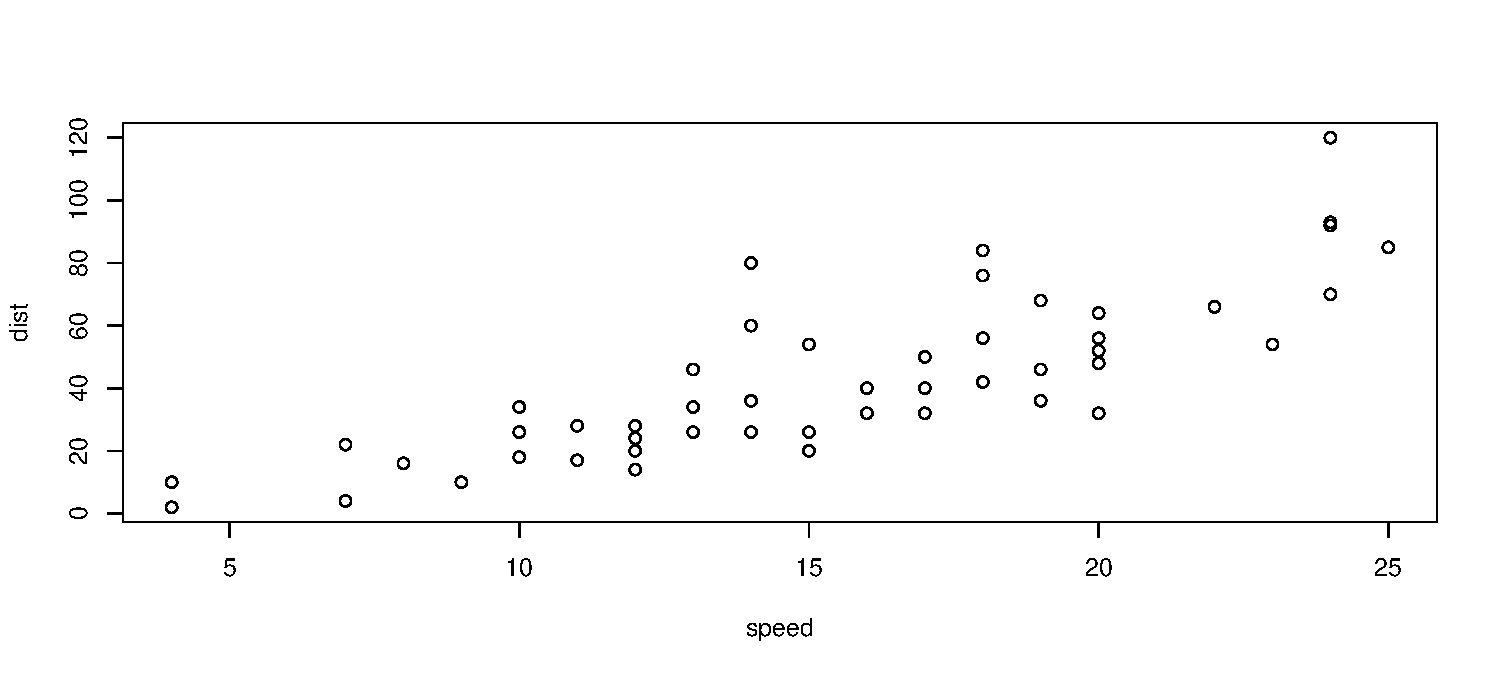
\includegraphics{bookdown-demo_files/figure-latex/my-chunk-1.pdf}
\caption{\label{fig:my-chunk}This is a long long long long caption.}
\end{figure}

\begin{Shaded}
\begin{Highlighting}[]
\FunctionTok{rnorm}\NormalTok{(}\DecValTok{10}\NormalTok{)}
\end{Highlighting}
\end{Shaded}

\begin{verbatim}
##  [1] -1.74060047  0.38711075 -0.58440161  2.45274348 -0.15456249 -0.64357430
##  [7]  0.04913925 -0.22799195  0.05917993  1.45417435
\end{verbatim}

  \bibliography{book.bib,packages.bib}

\end{document}
